\chapter{Advise on writing the thesis} \label{chap_writing}

The thesis is an own scientific work of the student. It will be read in any case by the first and second advisor, but it should be written in a way that it is understandable to anyone from the corresponding scientific area without the need to read additional literature. This holds in particular for employees of companies where the work has been carried out (in case of external theses).

\section{Number of pages}

It is not possible to give a general recommendation for the reasonable length of a thesis. This depends on the subject. For instance, a subject which includes a detailed comparison of related work may require more pages than a subject with a focus on the practical implementation. Table \ref{tab:pages} contains some suggestions for different kinds of theses.

% Tables can be put in a figure environment - the use of a table environment is in particular usefulif many tables are included
\begin{table}[htb]
  \centering
  \begin{tabular}{|l|p{3cm}p{3cm}p{3cm}|}
    \hline
    \textbf{Type of work} & \textbf{Minimum} & \textbf{Average} & \textbf{Maximum}\\ \hline
    Project report & 10 pages  + appendix (+ CD) & 15 pages + appendix (+ CD) & 30 pages  + appendix (+ CD)\\ \hline
    Bachelor thesis & 30 pages + appendix + CD & 45 pages + appendix + CD & 100 pages + appendix + CD\\ \hline
		Master thesis & 60 pages + appendix + CD & 75 pages + appendix + CD & 130 pages + appendix + CD \\
    \hline
  \end{tabular}
  \caption{Suggestions for the number of pages}\label{tab:pages}
\end{table}

Please note that the number of pages does not have an implication whether the thesis is good or bad (Einstein's PhD thesis had 17 pages). As discussed in the writing style section it is better to be precise and short rather than to describe something with many words.

\section{Writing style}

A thesis document is comparable to a research report or scientific book, like Tanenbaum's ``Computer Networks''. Scientific writing has to be a formal document - much more formal than many articles in the Internet. Colloquial and informal writing is undesirable.

Formal and informal English differ in word choice, word usage, and grammatical structures. Informal writing might utilize the words ``kid'', ``how come'' and ``quote'' as a noun. A formal writer might prefer ``child'', ``why'' and ``quotation'' \cite{sch96}. 

Non-native speakers should note that the word-by-word translations from another language like Chinese or German does not work in writing a thesis, so students are suggested to always use an English book as a reference for language.

Three keywords for scientific writing are \textit{clarity}, \textit{precision} and \textit{brevity}. They can serve as the watchwords to ensure a thesis is readable, persuasive and concise. Pages 18-26 in \cite{cha02} provide some very useful hints on understanding the three words and discusses some other issues on the use of language in thesis writing.

An important stylistic choice in scientific writing is between active voice and passive voice. One way to express what was done is to e.g.~say ``I performed frequency measurements''. In this way it becomes obvious what was done by the author. However, this kind of writing is uncommon in scientific work and should be used only when there would be uncertainties about who contributed which pieces of work. A better alternative writing to make this obvious is use a sentence similar to ``Frequency measurements were conducted by the author''. In most situations a passive form like ``Frequency measurements were conducted'' is the best option. 

In a scientific thesis it is very unusual to address the reader directly as ``you''. Thus, one should change sentences like ``This chapter tells you the reason why ...'' to ``This chapter gives reasons why ...''.

\section{Active verbs}

Using precise, active verbs can make the thesis more concise, precise and persuasive. For example, instead of saying ``This work is a generalization of Smith's earlier algorithm.'', it is better to write ``This work generalizes Smith's earlier algorithm.'' \cite{hew03}.

Some frequently used active verbs include: present, summarize, illustrate, clarify, reveal, introduce, indicate, propose, specify...

For more useful hints and a list of active verbs, please refer to \cite{hew03}.

\section{Transitional words and phrases}

Transitional words and phrases provide the glue that holds ideas together in writing. They help the reader to understand the relationships between ideas, and can be used to connect sentences, paragraphs, or even entire sections \cite{har11}.

The following paragraph is an example on how transitional expressions establish relationships between ideas and connect sentences to form a logical chain. In order to notice the difference read the paragraph with and without the words in \textit{italics}.

``\textit{Unlike} some common protocols \textit{such as} UDP, the original CCN protocol does not have any fixed-length fields in the messages. \textit{Instead}, the message formats are defined by XML schemas \textit{and} each field can be of arbitrary length ...

Such protocol design, \textit{however}, is not applicable to wireless sensor networks, which generally have very limited communication bandwidth. \textit{In particular}, the MAC layer frame size on our platform is merely 127 bytes ...''

Some more suggestions and a well-organized list of transitional words and phrases can be found in \cite{har11} and \cite{poss} (both online).

\section{Tenses}

Usually the thesis should be written in present tense. Sometimes it may be necessary to describe steps which have led to a current result. In this case it can be useful to use the past tense to explain the steps. It is important to use the tenses in a consistent manner.

\section{Formatting requirements}

The following layout settings are suggested for a thesis.
\begin{description}
\item[Paper:] A4
\item[Font:] Times New Roman 12pt or Arial 11pt; the font sizes should be at least 11 pt; no fancy fonts should be used
\item[Justification:] Use justification; avoid empty spaces by appropriate word separations
\item[Margins:] All around 2.5 cm (0.98 inches)
\item[Spacing:] one half spacing; is achieved by using the \textit{setspace} package 
\item[Page use:] single sided print for the two final printouts; the option \textit{oneside} in \textit{documentclass} is activated in this template 
\item[Tables:] For the table of contents, table of figures, etc there is no need to write them by hand. Use LaTeX commands to generate them automatically.
\end{description}

\section{Emphasis}

In scientific writing, there are several ways to highlight or emphasize some words or phrases within a paragraph, including \textbf{boldface}, \textit{italics}, \underline{underlining} and CAPITALIZATION. Generally speaking, boldface and italics are recommended while underling and capitalization should be avoided. However, even boldface and italics should be used \textit{sparingly} (especially boldface), because too many highlights will just do the opposite.

A student can use either boldface or italics or both in her or his writing, but the usage should be \textit{consistent} throughout the entire thesis. There is a subtle difference between boldface and italics. Within a large body of text, a word in \textit{italics} does not stand out much. Instead, it signifies a context difference only \textit{while} the text is being read. It is useful for highlighting the introduction of new terms. In contrast, a word in \textbf{boldface} can easily attract human eyeball and is therefore recommended for keywords that the readers might be looking for \cite{wik13a}.


\section{Citations} \label{sec_citations}

It is necessary to cite if foreign work has been included into the thesis. A reference has to be added which points to the bibliography and the bibliography has to contain enough information to find the sources. There are multiple standards on the format of citations. For scientific writing, the IEEE citation style is usually recommended. The detailed IEEE citation standard can be found online in \cite{ieeecitation09}. The BibTeX file belonging to this template contains examples for references to different sources.

The use of footnotes is possible, but is not recommended because it leads to a replication of information if the same source is cited multiple times (there may be a pointer to an earlier footnote to avoid this, but this solution is inconvenient for the reader). In addition, the use of footnotes disrupts the reader from the main text and is rather uncommon in electrical engineering or computer science documents in contrast to other scientific areas. 

Citations which use the wording of the foreign text need to be indicated with quotation marks. In electrical engineering and computer science word-by-word quotes are not useful in many cases and should be avoided. If they are used, they should be as brief as possible. It is preferable to explain something by using one's own words (it is of course still necessary to point to the source). One exception is the definition of important terms since an explanation using own terms may easily lead to a loss of precision. In this case the source needs to be provided with a detailed reference, e.g. indicating the page in a book.
 
When referencing Internet pages it needs to be taken into account that these may be changed over time. There should be a remark when they have been accessed for the last time. They should be downloaded (if possible) to make sure that the content is preserved.

\section{Figures and tables}

Figures and tables are always a good complement to the written text. They can visualize some complicated concepts or ideas, and help the readers understand the text better. Especially for those theses involving programming, a \textit{class diagram} can easily clarify the design of a program.

Similar to the use of boldface and italics, figures and tables should also be used \textit{sparingly} and \textit{selectively}. A common pitfall is to include too many screenshots in the thesis. Remember a thesis is basically a formal record of the author's original research, not a software tutorial or a user manual. Each figure has to provide an added value for the reader. This does not hold for company logos or startup screens.

Each figure or table should be labeled with a caption briefly stating its content. If the figure or table is taken from elsewhere, a reference has to be included in the caption as well.

Figures and tables are illustrations that complement the text. These illustrations can \textit{never} substitute text. Consequently, figures and tables need to be described and referenced in the text accordingly. A common pitfall is that students expect the reader to ``read'' the figures. A figure which is not referenced will may be considered by the reader, because she or he does not know when to look at the figure.

\section{Program code}

In computer-related books and articles, a piece of code is formally referred to as a listing or program listing. Similarly, program listings should also be used very sparingly, as all the source code will be available in the enclosed CD. Like figures and tables listings can only be used as a complement to the written text. Sometimes it is useful to explain something with a pseudocode rather than to provide all details of the actual code. 

Although there is no universal format for a listing, some basic rules should be followed. First, a listing should always be labeled, just like a figure or a table. Second, the font for the code should be mono-spaced (e.g. Courier New, etc.). Figure \ref{fig:examplecode} is a simple example of a listing (the format is not required but recommended).

\begin{figure}[htb]
  \centering
  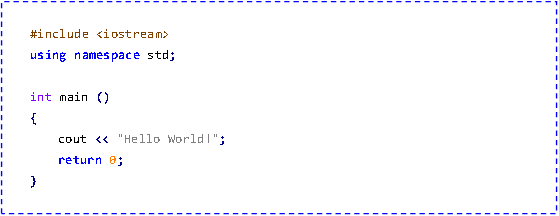
\includegraphics[width=.7\textwidth]{examplecode}
  \caption{Program listing example}\label{fig:examplecode}
\end{figure}

If a thesis contains only very few program listings, they might also be labeled as figures and included in the List of Figures. Otherwise, it is suggested to provide a List of Listings.

\lstset{emph={int,for},emphstyle=\normalfont \ttfamily\color{red},
backgroundcolor=\color{lightestyellow},
stringstyle=\normalfont \ttfamily,
basicstyle=\normalfont \ttfamily,
numbers=left}
\begin{lstlisting}[frame=trb,captionpos=b,caption=Display of program code using 1stlisting,label=lst:examplecode]
int $i;
for($i = 0; $i < 10; $i++) {
echo $i;
}
\end{lstlisting} 

Alternatively the program code can be shown by using a special LaTeX package named listings. The listing \ref{lst:examplecode} serves as an example.

If the thesis involves programming work, it is recommended to use code versioning software. In the material folder a Subversion tutorial is provided for this.

\section{Acronyms and terms}

The use of acronyms is common in scientific writing since it keeps the brevity of the text. However, when using an acronym for the first time, the phrase should be spelled out and followed by the acronym in parentheses (not in a footnote). Note that the phrase itself is usually in lower case. For example, wireless sensor networks (WSNs).

In order to avoid ambiguity it is not recommended to use different terms for the same concept. For instance, it may be unclear whether there are differences when terms like computer, machine, or device are used.

For bachelor or master theses it is not necessary to provide a glossary or a list of abbreviations. A key word index is also not useful.
 
\section{Spelling and grammar}

Spelling mistakes and wrong sentence structures give a bad impression and have to be avoided. In addition to the use of an automatic spell check further people should read the thesis when it is ready to be submitted. Otherwise, the readers may guess that not only the writing is inaccurate, but also the contents.

\endinput 